En la actualidad se ha vuelto un problema cotidiano encontrar un lugar disponible en un estacionamiento, principalmente en zonas comerciales, de oficinas o de gran actividad econ�mica. Es com�n que un conductor (usuario) vaya a un estacionamiento en espec�fico y no encuentre un espacio disponible, lo cual puede hacer que pierda un tiempo considerable en encontrar un lugar disponible. 

Una investigaci�n realizada por el Instituto de Pol�ticas para el Transporte y el Desarrollo (ITDP), revelo que en �reas d�nde la oferta de sestacionamientos no es suficiente para cubrir la demanda y se ofrecen espacios de estacionamiento en v�a p�blica de manera gratuita, se generan efectos negativos que afectan a residentes y visitantes. \cite{ITDP}.

\begin{figure}[h]
	\centering
	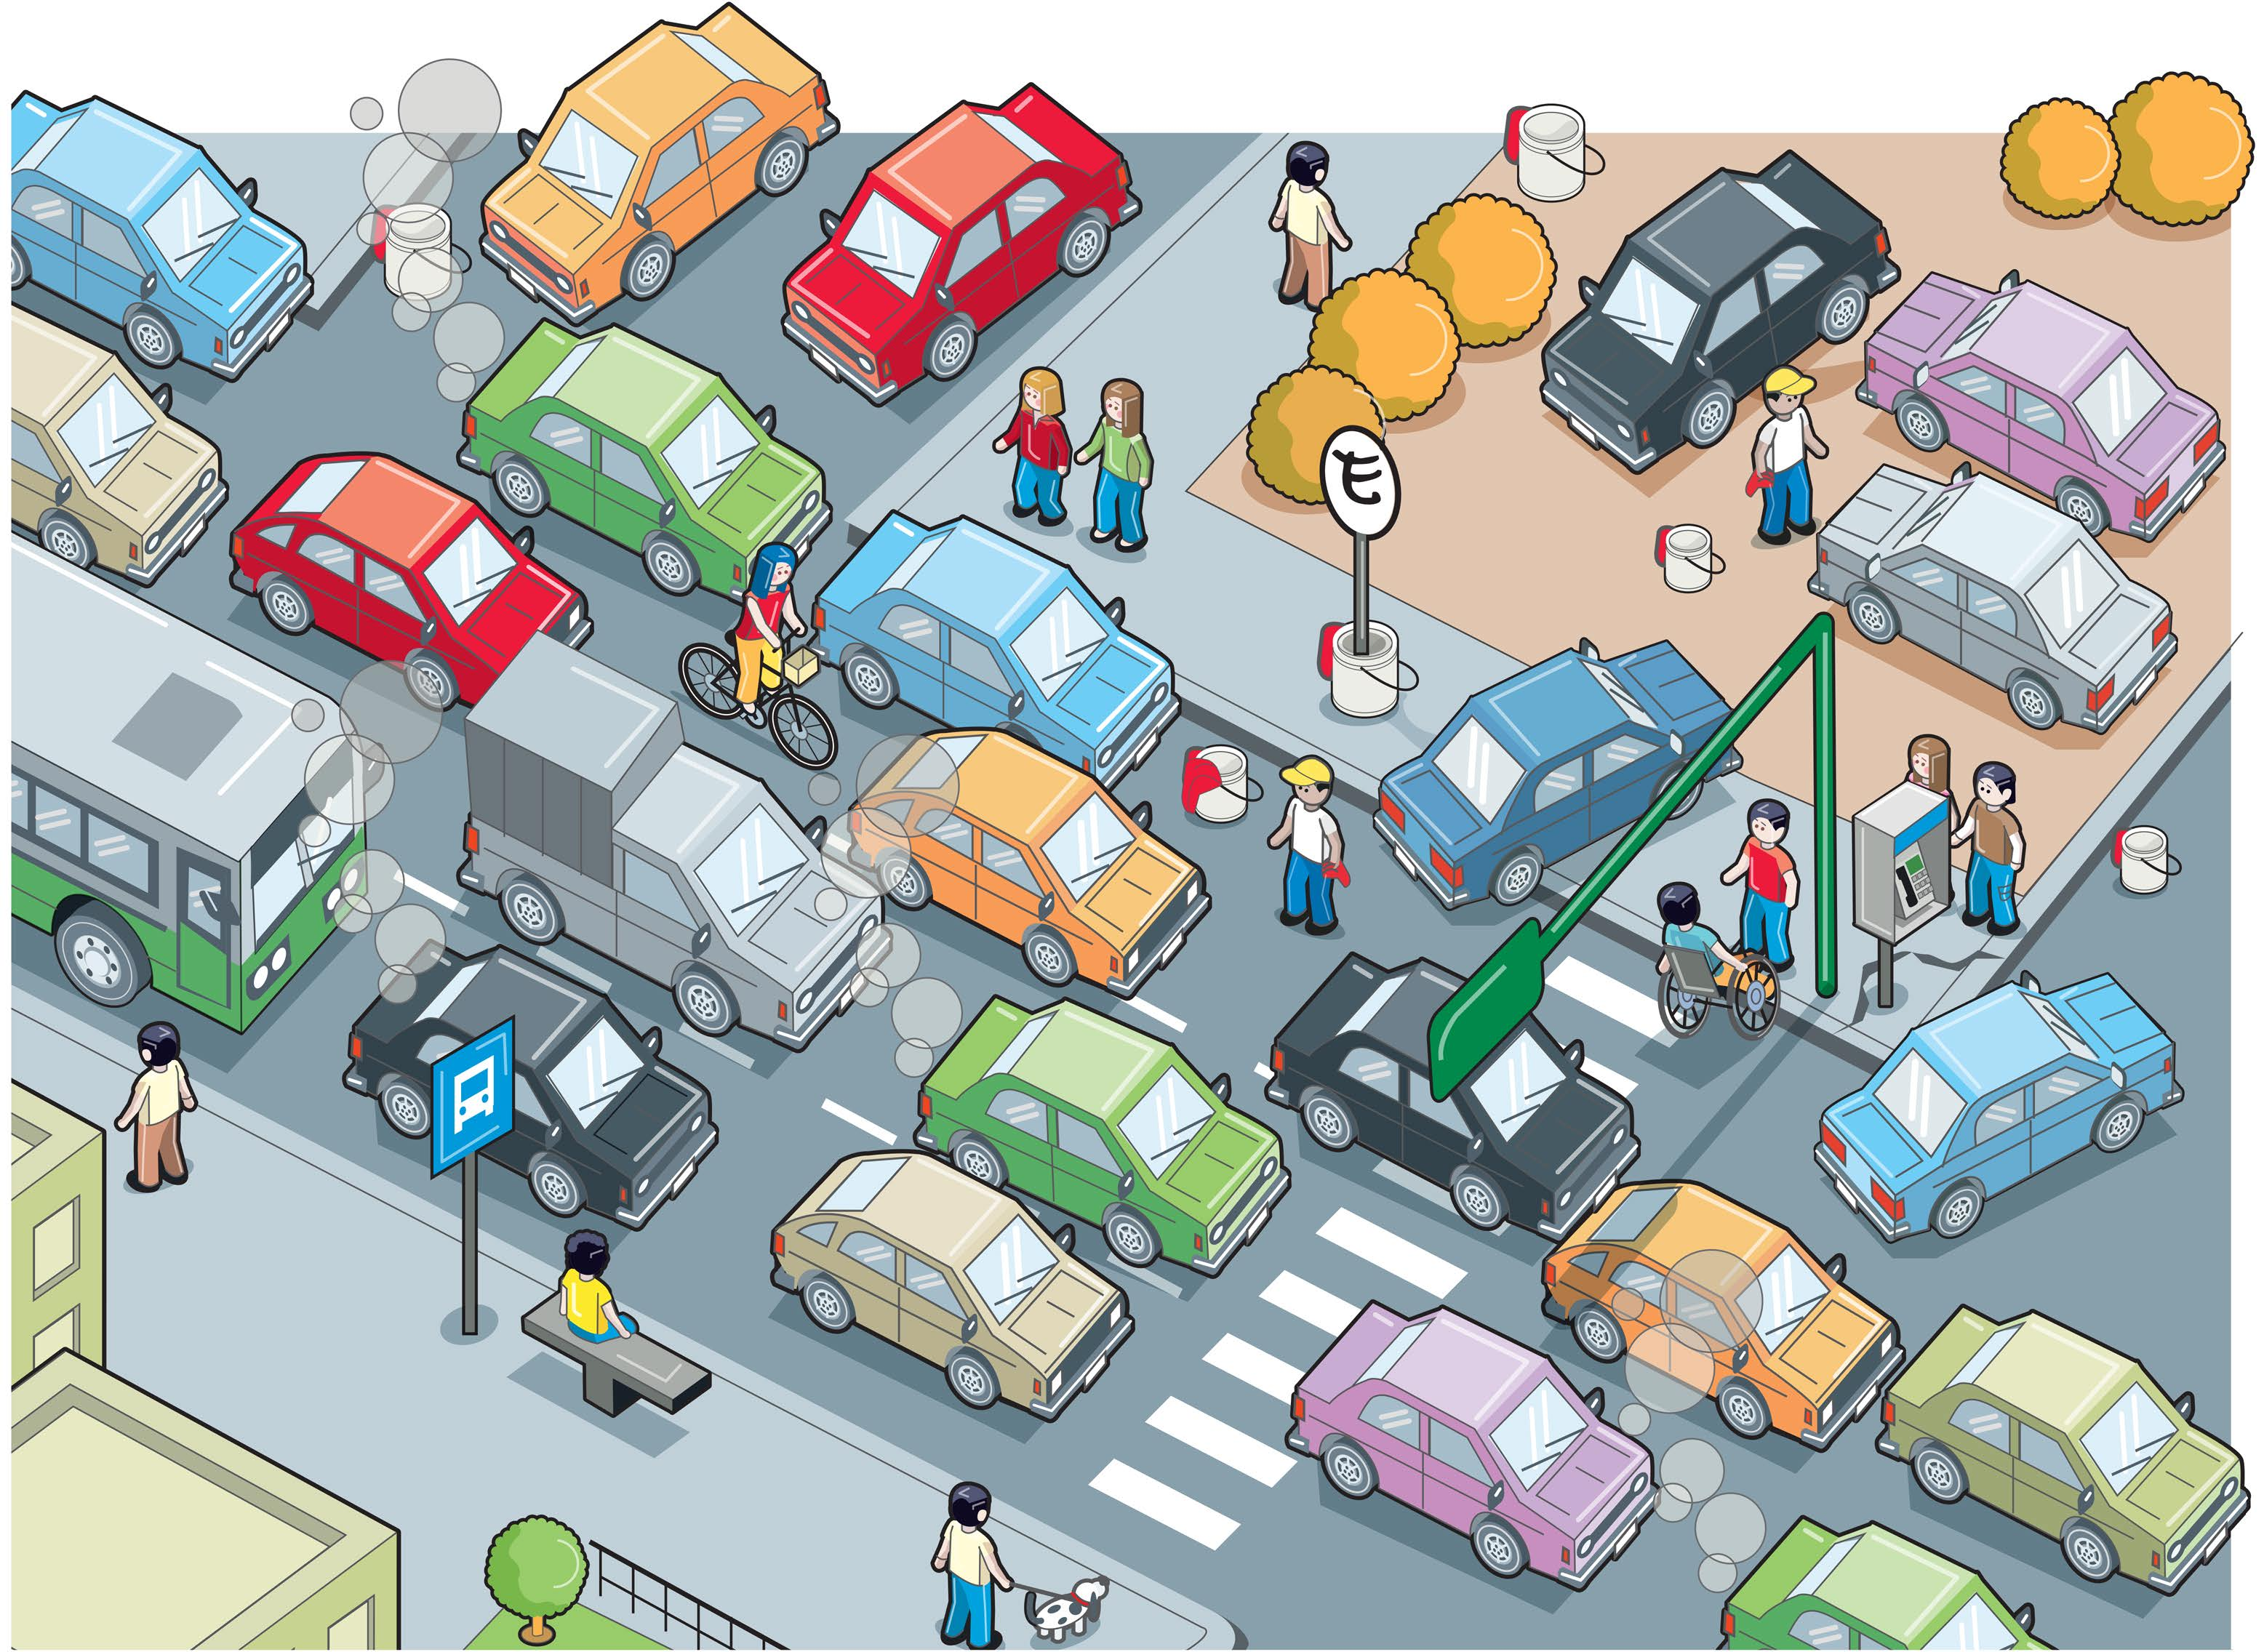
\includegraphics[scale=.25]{./definicionDelProblema/source/trafico.pdf}
	\caption{Problemas cotidianos por falta disponibilidad en estacionamietos}
	\label{fig:Tafico}
\end{figure}

\begin{itemize}
	\item Baja disponibilidad de estacionamientos
	\item Estacionamientos ilegales
	\item Apropiaci�n ilegal de estacionamientos
	\item Altos niveles de ruido y contaminaci�n
	\item Congesti�n vial y tiempos de b�squeda largos en estacionamientos	
\end{itemize}


Por otro lado en estacionamientos(administradores) peque�os y medianos los ingresos no son suficientes para la adquisici�n de un sistema o la contrataci�n de  un  agente  externo  que  realice  dichas  administraci�n;  incluso  para  estacionamientos  grandes  con  mayores  ingresos  la implementaci�n de un sistema, automatizaci�n u outsourcing disminuye en gran medida sus ingresos.